\documentclass{fithesis}


\usepackage{listings}
\usepackage{lmodern}
\usepackage[czech]{babel}
\usepackage[utf8]{inputenc}
\usepackage{cmap}
\usepackage{graphicx}
\usepackage[T1]{fontenc} %formátuje české znaky - důležité
\usepackage[plainpages=false, pdfpagelabels]{hyperref}
\usepackage{hyperref}
\usepackage{longtable}
%\usepackage{makeidx}
%\makeindex
\def\figureautorefname{Obrázek}%
\def\tableautorefname{Tabulka}%
\def\lstlistingname{Ukázka kódu}%
\def\sectionautorefname{Kapitola}%
\usepackage{listings}
\usepackage{color}
 
\definecolor{codegreen}{rgb}{0,0.6,0}
\definecolor{codegray}{rgb}{0.5,0.5,0.5}
\definecolor{codepurple}{rgb}{0.58,0,0.82}
\definecolor{backcolour}{rgb}{1,1,1}
 
\lstdefinestyle{mystyle}{
    backgroundcolor=\color{backcolour},   
    commentstyle=\color{codegreen},
    keywordstyle=\color{magenta},
    numberstyle=\tiny\color{codegray},
    stringstyle=\color{codepurple},
    basicstyle=\footnotesize,
    breakatwhitespace=false,         
    breaklines=true,                 
    captionpos=b,                    
    keepspaces=true,                 
    numbers=none,                    
    numbersep=5pt,                  
    showspaces=false,                
    showstringspaces=false,
    showtabs=false,                  
    tabsize=2
}
 
\lstset{style=mystyle}



\lstdefinelanguage{JavaScript} {
	morekeywords={
		break,const,continue,delete,do,while,export,for,in,function,
		if,else,import,in,instanceOf,label,let,new,return,switch,this,
		throw,try,catch,typeof,var,void,with,yield
	},
	sensitive=false,
	morecomment=[l]{//},
	morecomment=[s]{/*}{*/},
	morestring=[b]",
	morestring=[d]'
}



%\bibliographystyle{unsrt}


%\makeindex
\thesistitle{Integrace DMS a workflow v Liferay Portal}
\thesissubtitle{Diplomová práce}
\thesisstudent{Bc. Marek Tlačbaba}
\thesiswoman{false}
\thesisfaculty{fi}
\thesisyear{2014}
\thesisadvisor{RNDr. Jaroslav Ráček, Ph.D.}


\begin{document}

\FrontMatter
\ThesisTitlePage

\begin{ThesisDeclaration}
Prohlašuji, že tato práce je mým původním autorským dílem, které jsem
vypracoval samostatně. Všechny zdroje, prameny a literaturu, které jsem při vypracování používal nebo z nich čerpal, v práci řádně cituji s uvedením
úplného odkazu na příslušný zdroj.\AdvisorName
\end{ThesisDeclaration}

\begin{ThesisThanks}
Na tomto místě bych chtěl poděkovat vedoucímu práce RNDr. Jaroslavu Ráčkovi, Ph.D. a vývojářům ze společnosti IBA CZ za konzultace a informace při vytváření této práce. Také bych rád poděkoval své rodině a blízkým za zázemí, které mi během práce poskytli.
\end{ThesisThanks}

\begin{ThesisAbstract}
Cílem práce je seznámit se s problematikou podnikových portálů a s tvorbou portletů. Praktickým výstupem práce je implementace grafického workflow editoru pro tvorbu workflow v Liferay Portal verze CE. Práce se nejprve věnuje obecně podnikovým portálům a vývoji portletů. Následuje část věnující se workflow systémům a notaci BPMN. Pak následuje srovnání podobných řešení pro jiné systémy a jsou vyspecifikovány požadavky na novou aplikaci. Je popsána architektura aplikace a technologie použité při realizaci. Pozornost je věnována především rámci Spring, frameworku Alloy UI, nástroji JAXB a portálovému API. Dále je popsáno provedené testování aplikace a~uživatelská dokumentace.
\end{ThesisAbstract}

\begin{ThesisKeyWords}
Podnikový portál, portlet, Java, Liferay Portal, workflow, Spring MVC, Alloy~UI
\end{ThesisKeyWords}


\MainMatter
\setcounter{secnumdepth}{4}
\tableofcontents

\chapter{Úvod}
Dnešní společnosti se stále snaží zlepšit svoji efektivitu zaváděním nových počítačových systémů. Stále častěji se nasazují takzvané podnikové portály, které zajišťují jednotný přístup k aplikacím, informacím a dokumentům přehledně z jednoho místa.

Právě práce s dokumenty je v podnicích často klíčová činnost a potřeba řídit jejich tok je zásadní. Za tímto účelem jsou v podnikových portálech používané workflow systémy, které jsou používané k řízení podnikových procesů včetně řízení toků dokumentů. Podnikový portál Liferay Portal obsahuje vlastní workflow systém Kaleo. Do tohoto systému je možné vkládat nové definice workflow pouze pomocí dokumentů ve formátu XML, které mají přesně definovanou strukturou. Právě tvorba těchto definic je vhodná pouze pro odborníky a pro méně technicky zdatné pracovníky bývá často neřešitelný problém vytvořit nové definice. Cílem této diplomové práce je vytvořit grafický workflow editor, který bude napojen na workflow systém Kaleo v~portálu Liferay Portal a bude umožňovat tvorbu workflow definicí v~základní notaci BPMN. Tento grafický workflow editor bude vytvořen jako klasická portletová aplikace, která půjde klasickou cestou nasadit do portálu Liferay a bude přístupná pro administrátory portálu. Editor umožní vytvářet, upravovat a vkládat definice do workflow systému v portálu. Takto vložené definice již bude možné využít v portálu standardním způsobem a~budou tedy dostupné i při řízení toků vnitropodnikových dokumentů. Pro vývoj budou použity moderní technologie platformy Java EE. Práce bude řešena v rámci Sdružení průmyslových partnerů Fakulty informatiky pro společnost IBA CZ.

První kapitola se věnuje portálům obecně, jejich vlastnostem a konkrétním portálovým platformám. Blíže jsou analyzovány možnosti portálu Liferay.

Druhá kapitola se věnuje vývoji portletů, tedy aplikacím běžícím v prostředí portálů. Je zde popsán základní účel portletů, existující standardy pro vývoj portletů v jazyku Java, infrastruktura portálu a hlavní aspekty týkající se vývoje portletů.

Třetí kapitola se věnuje systémům workflow, jejich dělením a obecnému modelu workflow. V této kapitole je také popsána základní notace BPMN pro modelování podnikových procesů. Blíže jsou zde popsány ty elementy, které jsou podporovány workflow systémem Kaleo používáným v portálu Liferay.

Čtvrtá kapitola se zabývá analýzou požadavků na vytvářený workflow editor. Nejprve je provedeno srovnání s existujícími řešeními a následně jsou sestaveny skupiny požadavků na nový editor.

Pátá kapitola je věnována realizaci vytvářené aplikace. Je zde popsána architektura a technologie použité při implementaci.

Šestá kapitola popisuje provedené testy, které byly zvoleny pro ověření kvality vytvořené aplikace. 

V sedmé kapitole je popsána dokumentace ke vzniklé aplikaci.







\chapter{Podnikové portály}
Pojem portál bývá definován různými způsoby v závislosti na situaci, ve které je používán. Dříve se portály zaměřovaly na jednotný přístup k informacím nezávisle na jejich původu a umístění. S~dalším vývojem informačních technologií se postupně tento přístup rozšiřoval a~do definice portálu přibyly pojmy jako integrace a agregace služeb a aplikací. V následujícím textu je uvedeno několik definic portálu a také podnikového portálu.

Například Gála definoval portál jako jednotné rozhraní, ve kterém lze pracovat s běžnými službami a nástroji jako jsou, například zpravodajství a~komunikace, mimo to je v něm zaručen přístup k všeobecným aplikacím jako jsou vlastní stránky a blogy, a k aplikacím specializovaným, například slovníkům. \cite{gala}

Další definice portálu je převzata ze standardu JSR--286. Portál je webová aplikace, která (obvykle) poskytuje možnost personalizace, autentifikace, agregace obsahu z různých zdrojů a slouží jako prezentační vrstva informačních systémů. Agregací se rozumí integrace obsahu z různých zdrojů v~rámci jedné webové stránky. Portál může mít vysoce propracované nástroje pro personalizaci, které poskytují obsah upravitelný podle přání uživatele. Stránky portálu mohou mít různé skupiny portletů \footnote[1]{Bližší informace v dalších částech této práce.}, které vytvářejí obsah pro různé uživatele.  \cite{jsr-286}

Předchozí definice se týkají portálu obecně, proto zde uvedu také definici podnikového portálu. Podle Čecha je podnikový portál definován jako internetové nebo intranetové stránky, které slouží jako vstupní bod, respektive brána k různým datovým, informačním a znalostním zdrojům v organizaci. Jejich cílem je zpřístupnit tyto zdroje specifické skupině lidí. Může to být jak zákazníkům, tak také vlastním zaměstnancům nebo partnerům. \cite{cech}

V předchozích definicích portálu jsou naznačeny některé základní rysy podnikových portálů. Mezi důležité vlastnosti považujeme jediný přístupový bod, integrace, federace, přizpůsobivost, personalizace, kontrola přístupu a~vyhledávání v podnikovém obsahu.\cite{enterprise-portal}

\section{Konkrétní portálová řešení}
Existuje a používá se celá řada konkrétních portálových řešení. Nejčastěji však bývají implementovány v jazyce Java a podporují standardy JSR--168 a~JSR--286~\footnote[2]{Bližší informace v dalších částech této práce} pro tvorbu portletů v jazyce Java. Existují také portály pro jiné technologie, například pro platformu .NET je možné využít Microsoft SharePoint, ale nejvíce řešení existuje pro jazyk Java, kde mezi nejznámější patří IBM Websphere Portal, JBoss GateIn, Oracle WebCenter či Liferay Portal. Tyto portály již většinou obsahují velké množství připravených portletů, např. wiki stránky, správu souborů, portlety pro komunikaci a mnohé další.

\section{Liferay Portal}
Liferay Portal je open source podnikový portál založený na jazyce Java vyvíjený společností Liferay, Inc.. Podporuje specifikace JSR-168 a JSR-286 pro tvorbu portletů v jazyce Java. Liferay Portal je k dispozici ve dvou edicích, Community Edition (CE) a Enterprise Edition (EE).

Liferay Portal CE je bezplatná verze portálu, která je volně dostupná ke stažení. Tato verze neobsahuje oficiální podporu, která je zde poskytovaná pouze prostřednictvím Liferay komunity. Druhá verze portálu, Liferay Portal EE, je již placená edice. U této edice je kladen velký důraz na stabilitu, bezpečnost, výkon a patří k ní dlouhodobá podpora od společnosti Liferay, Inc. nebo jejích oficiálních partnerů.

Ihned po instalaci portálu je k dispozici množství již předinstalovaných portletů. Je možné například okamžitě využívat wiki stránky, fórum, kalendář či galerii obrázků. Liferay podporuje různé způsoby úprav či rozšíření. Pro změny vzhledu můžeme využít témata či šablony, další funkcionalitu portálu je možno přidávat pomocí portletů. Pro změnu chování portálu či portletů se používají tzv. hooks. Pokud se jedná o větší a zásadnější změny přímo v jádru portálu, ty jsou prováděny pomocí pluginu Ext. \cite{developer-guide}

Portál Liferay nabízí svým uživatelům zabezpečené jednotné přihlášení, nástroje pro správu workflow, snadnou instalaci samotného portálu i dalších nových aplikací a rozšíření. Od verze 6.1 umožňuje instalaci rozšíření a~aplikací nově také z Liferay Marketplace. Takto je možné stahovat aplikace přímo z rozhraní portálu a jednoduše je přidat do portálu.

Liferay také obsahuje pokročilý systém pro správu obsahu (Liferay CMS), který umožňuje oprávněným uživatelům vytvářet a spravovat obsah webu přímo z prohlížeče a to i bez znalosti programování. S tím také souvisí možnost dělit uživatele do organizací, skupin a uživatelům přidělovat role, podle kterých jim následně zobrazovat různý obsah, aplikace a umožňovat provádět různé akce.

Mezi další vlastnosti portálu patří vícejazyčné uživatelské rozhraní, personalizace portálových stránek, jednoduchá úprava stránek způsobem táhni a pusť, automatické nahrávání souborů.

Liferay také podporuje různé platformy a proto je možné ho provozovat na různých aplikačních serverech, operačních systémech a databázích. Také podporuje různé metody integrace včetně SOAP, REST, RSS a také další proprietární rozhraní.\cite{liferay-features}

To jsou některé z důvodů, proč se podnikový portál Liferay stal rozšířenou a oblíbenou platformou pro vývoj firemních webů a systému v jazyce Java. Výběr portálu Liferay CE pro účely této práce vyplývá ze zadání práce a~potřeb společnosti IBA CZ.


\chapter{Vývoj portletů}
V této kapitole bude popsán vývoj portletů, které tvoří obsah portálů.

\section{Portlet}
Portlet je webová aplikace, která poskytuje uživatelům specifický obsah, typicky informaci nebo službu. Portlet je spravován portletovým kontejnerem, který zpracovává požadavky portletu a následně generuje dynamický obsah v podobě fragmentů v některém ze značkovacích jazyků -- HTML, XHTML, WML. Tyto fragmenty jsou pak spojovány a dohromady vytváří portálovou stránku.

Portletový kontejner má tedy odpovědnost za řízení životního cyklu jednotlivých portletů a je v něm také uloženo nastavení uživatele pro daný portlet. Ale části generované jednotlivými portlety slučuje dohromady na stránku portál. Portál a portletový kontejner mohou být postaveny jako jedna komponenta, ale mohou to být také komponenty dvě. Na obrázku \ref{fig:vytvareni_stranky} je zobrazen průběh vytváření stránky v portálu tak, jak bylo výše naznačeno.

\begin{figure}[htp]
\centering
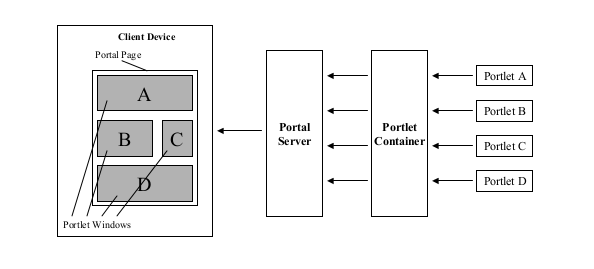
\includegraphics[width=340px]{images/vytvareni_stranky_v_portalu.png}
\label{fig:vytvareni_stranky}
\caption{Vytváření stránky v portálu (převzato z \cite{jsr-286})}
\end{figure}

\section{Portletová specifikace}
Důvodem pro vytvoření portletové specifikace byla situace, kdy různí dodavatelé používali svá vlastní API, která neumožňovala přenositelnost mezi portálovými servery.

První verze Java Portlet Specification 1.0 (JSR-168) byla vydána v roce 2003. V této specifikaci ještě byly různé nedostatky a chyby, které pak tvůrci portletů stejně řešili každý po svém. To i nadále způsobovalo, že portlety byly mezi portálovými servery stále problematicky přenositelné či nepřenositelné úplně. Proto vznikla druhá verze Java Portlet Specification 2.0 (JSR-286) a~ta byla vydána v červnu 2008. Mezi nejdůležitější přínosy patří následující:
\begin{itemize}
\item sdílení parametrů mezi portlety skrz veřejné render parametry,
\item meziportletová komunikace pomocí zasílaní událostí,
\item transformace informací nově definovanými portletovými filtry,
\item možnost portletů poskytovat zdroje jako jsou například PDF soubory.
\end{itemize}
Většina portletových kontejnerů poskytuje k základním požadavkům i svá vlastní rozšíření, která však  nemusíme využívat a tím můžeme zachovat myšlenku snadné přenositelnosti.

\subsection*{Životní cyklus portletu}
Každý portlet musí implementovat rozhraní \verb|Portlet|. Toto rozhraní obsahuje čtyři základní metody, které musí být implementovány a které řídí životní cyklus portletu - \verb|init(), processAction(), render(), destroy()|.

Metoda \verb|init()| je volána ihned při vytváření portletu a je používána například pro přípravu zdrojů potřebných portletem.

Metoda \verb|processAction()| je volána vždy po provedení nějaké akce uživatelem, pokud se touto akcí nějak mění stav portletu. Může to být například akce potvrzení formuláře a následné zpracování a uložení dat v databázi.

Metoda \verb|render()| má za úkol generovat fragment stránky, který je pak dostupný uživateli v portletu. V této metodě by se neměl měnit stav portletu.

Poslední metodou je \verb|destroy()|. Ta je volána před odstraněním portletu z paměti. Poskytuje poslední možnost pro uvolnění zdrojů, které byly portletem používány. \cite{jsr-286}
\clearpage

Zpracování požadavků v portletech může procházet několika fázemi zpracování.

\begin{itemize}
\item Render -- vykreslovací fáze, ve které se typicky nemění stav portletu, odpovídá jí metoda \verb|render()|.
\item Action -- portlet zpracovává nějakou akci a typicky mění svůj stav, odpovídá ji metoda \verb|processAction()|.
\item Resource -- portletem je poskytován nějaký zdroj, např. PDF soubory. Aby portlet mohl podporovat tuto funkcionalitu, musí implementovat rozhraní \verb|ResourceServingPortlet|.
\item Event -- portlet přijímá nějakou událost a nějak na ni reaguje. Portlet v tomto případě musí implementovat rozhraní \verb|EventPortlet|.
\end{itemize}

Všechny tyto rozhraní implementuje abstraktní třída \verb|GenericPortlet|. Tato třída obsahuje implementaci všech povinných metod a několika dalších, které je možné využít.

Po každé action fázi musí následovat fáze render. Pokud se na portálové stránce vyskytuje více portletů, je metoda render zavolána u všech zobrazených portletů. 

\subsection*{Režimy portletu}
Portletová specifikace obsahuje tři režimy portletu, které umožňují zobrazit jiný obsah v závislosti na požadovaném úkolu. Tyto režimy využívá metoda \verb|render()|, která podle nich vygeneruje odpovídající obsah.

\begin{itemize}
\item View -- základní režim používaný při klasickém zobrazení portletu na portálové stránce.
\item Edit -- nepovinný, uživateli umožňuje nastavovat portlet.
\item Help -- nepovinný, zobrazuje se nápověda k danému portletu.
\end{itemize}

Ve třídě \verb|GenericPortlet| jsou k těmto účelům definovány tři metody \verb|doView()|, \verb|doEdit()| a \verb|doHelp()|. Jednotlivé portletové režimy by měly být implementovány přetížením těchto metod. Každý portál si také může definovat vlastní portletové režimy. Každý portlet musí mít zadefinováno, které režimy podporuje.

\subsection*{Stavy okna}
Portletová specifikace definuje tři základní stavy.

\begin{itemize}
\item Minimized -- okno portletu je minimalizované.
\item Normal -- původní velikost portletu, které umožňuje zobrazení všech portletů na na portálové stránce.
\item Maximized -- okno portletu skryje ostatní portlety na stránce a zobrazuje se pouze tento maximalizovaný portlet, nebo zakrývá většinu dostupné plochy.
\end{itemize}

\subsection*{Struktura portálové aplikace}
Portálové aplikace jsou uloženy ve standardní archivním souboru jazyka Java, Web ARchive (WAR). Mohou obsahovat více portletů, servlety, JSP soubory a další. Musí obsahovat webový deskriptor a také navíc portletový deskriptor implementace \verb|portlet.xml|.


















\chapter{Workflow}
Jednoznačná definice workflow neexistuje, jelikož každá oblast, ve které je workflow používáno, si ho definuje po svém. Obecně je ale možné definovat workflow jako proces automatizace podnikových procesů. O sjednocení této terminologie se již v roce 1996 pokusil institut Workflow Management Coalition (WfMC), kdy vydal terminologický slovník. V tomto slovníku workflow znamená automatizaci celého nebo části podnikového procesu, během kterého jsou dokumenty, informace nebo úkoly předávány od jednoho účastníka procesu k druhému podle sady procedurálních pravidel tak, aby se dosáhlo nebo přispělo k plnění celkových/globálních podnikových cílů. \cite{wfmc}

V počítačových systémech je workflow definováno jako systém řízení workflow. V tomto systému je možné workflow definovat, vytvořit a celý průběh procesu řídit. Mezi jeho úkoly patří provádět definici procesu, komunikovat s účastníky workflow, případně spouštět další aplikace nutné k~vykonání workflow.


\section{Typy workflow systému}
Workflow systémy se mohou dělit do několika skupin podle různých hledisek či typů. \cite{workflow}

\subsection*{Hledisko charakteru procesů}
\begin{itemize}
\item \textbf{Administrativní} workflow systémy jsou určeny k vyřizování běžných administrativních úkonů, které jsou většinou jednoduché, opakující se a dobře strukturované.
\item \textbf{Ad-hoc} workflow systémy jsou založeny na náhodnosti vzniku. Procesy bývají jedinečné a je nutné je definovat až při jejich vzniku.
\item \textbf{Kolaborativní} workflow systémy podporují především týmovou spolupráci. Zde je typickým znakem existence nějakého dokumentu, skrze který si uživatelé vyměňují poznatky a většinou se tento dokument stává i výsledkem společné práce. Často obsahuje opakovaní několika iterací stejného kroku dokud nedojde ke shodě.
\item \textbf{Produkční} workflow systémy podporují hlavní podnikové procesy, které vytvářejí přidanou hodnotu k finálnímu produktu.
\end{itemize}

\subsection*{Hledisko orientace procesů}
\begin{itemize}
\item \textbf{Procesy orientované na lidi.} U těchto systémů spoléhají účastníci sami na sebe. Předávané informace jsou proměnlivé a procesy nejednotné a špatně předpověditelné. Z těchto důvodů jsou průběhy závislé na jednotlivcích.
\item \textbf{Procesy orientované na sebe.} Tyto systémy jsou zaměřené na klíčové procesy, které obvykle bývají hlavními aktivitami podniku. Jejich pravidla řešení a jejich zpracování jsou pevně daná.
\end{itemize}

\subsection*{Hledisko technologické infrastruktury}
Podle technologické infrastruktury, nad kterou je systém workflow postaven, lze produkty rozdělit do několika skupin.
\begin{itemize}
\item Založené na \textbf{elektronické poště} -- využívají dostupné emailové servery. Uživatelé nepotřebují speciální software.
\item Založené na \textbf{procesech} -- mohou implementovat vlastní komunikační mechanismus a jsou postaveny na určitém databázovém systému. Bývají tvořeny jako komplexní řešení uceleného konceptu workflow.
\item Založené na \textbf{webu} -- využívají jednotného rozhraní intranetové aplikace. Je to univerzální platforma pro sdílení informací.
\item Založené na \textbf{dokumentech} -- tyto systémy byly motivovány představou o směrování dokumentů. Využívají systémy pro správu dokumentů.
\end{itemize}

\section{Obecný model workflow systému}
Institut WfMC vytvořil obecný model, kde mají produkty podobné komponenty. Tento model můžeme vidět na následujícím obrázku \ref{fig:obecny_model_workflow} a podle tohoto modelu se  jednotlivé komponenty systému dělí na programové a datové.

\begin{figure}[htp]
\centering
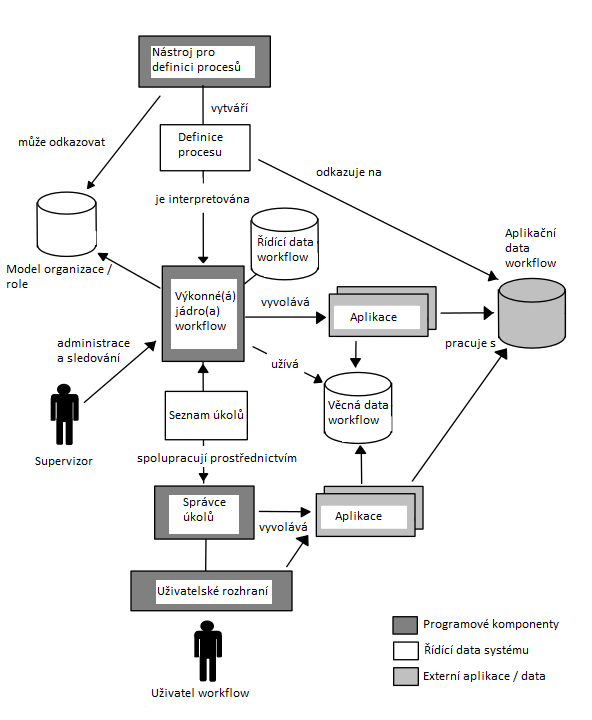
\includegraphics[width=340px]{images/obecny_model.png}

\caption{Obecný model workflow (převzato z \cite{wfmc})}
\label{fig:obecny_model_workflow}
\end{figure}


\subsection*{Programové komponenty}

\begin{itemize}
\item Nástroj pro definici procesů umožňuje definovat procesy, přiřazovat role a stanovat pravidla.
\item Výkonné jádro workflow řídí průběh workflow procesů, spouští nutné externí aplikace a udržuje statistiky o průběhu workflow.
\item Správce úkolů má jako hlavní úkol zprostředkovávat komunikaci mezi jádrem workflow a jednotlivými uživateli.
\item Uživatelské rozhraní zajišťuje komunikaci mezi správcem úkolů a uživatelem. Často tvoří jeden celek spolu se správcem úkolů.
\end{itemize}

\subsection*{Datové komponenty}

\begin{itemize}
\item Definice procesu popisuje strukturu procesu.
\item Řídící data workflow jsou interní data, které zpracovává jádro systému.
\item Aplikační data workflow jsou specifická data aplikací.
\item Věcná data workflow jsou data používaná jádrem k vyhodnocování dalších kroků.
\item Seznam úkolů představuje datovou strukturu, ve které jsou uloženy úkoly pro uživatele. Mohou být viditelné všechny najednou, nebo mu úkoly mohou být poskytovány postupně.
\item Model organizační struktury popisuje organizační strukturu podniku. Pokud není definován, musí být úkoly přiřazovány pouze konkrétním uživatelům.
\end{itemize}

\subsection*{Fáze workflow}
Obecně jsou rozlišovány dvě fáze workflow: fáze návrhu workflow a fáze průběhu workflow. \cite{workflow}

Fáze návrhu workflow v sobě zahrnuje funkce pro návrh a definici procesu, které jsou poskytovány analytickými a modelovacími nástroji. Ty umožňují převod procesu z reálného světa do normalizované podoby. Výsledkem je počítačově zpracovatelný popis procesu ve smyslu: kdo, kdy, co, s čím, za jakým účelem a jak má udělat.

Fáze průběhu workflow se dále dělí na funkce pro řízení běhu procesu, které zabezpečují interpretaci procesu, spouštění, provádění a kontrolu průběhu jednotlivých činností. Další část této fáze představuje interakce s uživateli a aplikačními nástroji. To například znamená předávání úkolů ke zpracování, vyžádání manuální činnosti, automatické spouštění jiných aplikací či předávání dat mezi aplikacemi. Vše je znázorněno na obrázku \ref{fig:faze_workflow_obr}.

\begin{figure}[htp]
\centering
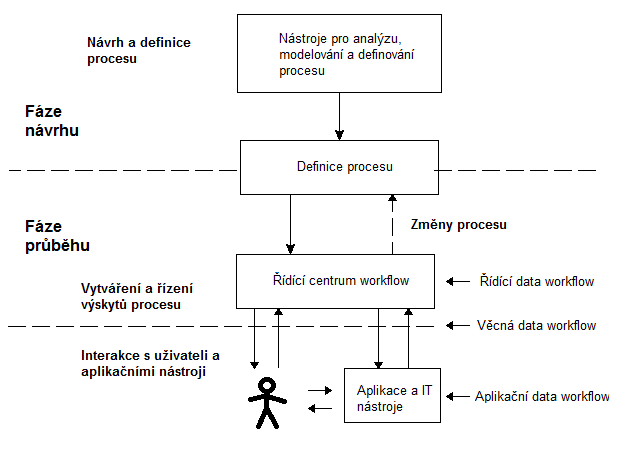
\includegraphics[width=340px]{images/faze_workflow.png}
\caption{Fáze workflow (převzato z \cite{wfmc})}
\label{fig:faze_workflow_obr}
\end{figure}

\section{Workflow pro procesy pracující s dokumenty}

Z pohledu charakteru procesů řadíme workflow pro procesy pracující s dokumenty do administrativních workflow. Většinou jsou to již procesy ustálené, dobře strukturované a tyto procesy jsou využívány většinou uživatelů systému. Z hlediska technologické infrastruktury jsou to systémy založené na dokumentech. Z hlediska orientace procesů patří do procesů orientovaných na sebe, jsou pro něj totiž typické vlastnosti jako předpověditelnost, strukturovanost, stálý postup a je aktivován dokumenty.






\section{BPMN}
Buisiness Process Model And Notation (BPMN) je standard pro modelování podnikových procesů, jehož výstupem bývá grafické znázornění podnikových procesů v podobě procesních diagramů. \cite{bpmn} Jazyk BPMN pomáhá sjednocovat významy základních pojmů používaných v této oblasti procesního řízení. 

Hlavním účelem BPMN je podporovat procesní řízení. Pro tuto funkci poskytuje notaci, která je jednoduchá, srozumitelná a intuitivní i pro netechnické pracovníky a zároveň dostatečná i pro vyjádření komplexních procesů. Přináší tedy standardizovaný zápis ve srozumitelné podobě pro všechny zainteresované osoby v organizacích.

Poslední verze BPMN 2.0 byla vydána v lednu 2011 a klade si za cíl být jedinou notací pro tvorbu modelů podnikových procesů. Proto mezi základními rysy jsou:
\begin{itemize}
\item snaha vytvořit jednotný konzistentní jazyk sjednocením definice podnikových procesů BPMN,
\item možnost vytvořit nezávislý nebo integrovaný model,
\item podpora a možnost výměny odlišných pohledů na procesní model tak, že je možno se v procesu zaměřit na slabá místa,
\item poskytnout xml schémata sloužící pro transformaci modelů.
\end{itemize}

Objekty jazyka BPMN jsou děleny do těchto základních kategorií. Tokové objekty, spojovací objekty, plavecké dráhy a artefakty. \cite{bpmn} Workflow systém Kaleo umožnuje využít pouze tokové objekty a základní spojovací objekty.

\subsection*{Tokové objekty}
Bývají označovány jako hlavní grafické prvky definující firemní procesy a~dále je možné je dělit například tak, jak je vidět na obrázku \ref{fig:tokove_objekty}.
\begin{itemize}
\item Události představují děje či události, ke kterým dochází v průběhu procesu. Na zmíněném obrázky to jsou objekty: Start, Stav a Konec.
\item Aktivity vyjadřují činnosti, které se odehrávají uvnitř procesu. Ty se dále dělí úlohy a podprocesy. Je to objekt: Úloha.
\item Brány jsou využívány pro zobrazení větvení a slučování toků a procesů, kdy je potřeba zohlednit různé podmínky. Jsou děleny na exkluzivní, inkluzivní a paralelní. Jsou to objekty: Podmínka, Větvení a Spojení.
\end{itemize}

\begin{figure}[htp]
\centering

\includegraphics[width=340px]{images/tokove_objekty.png}
\caption{Tokové objekty používané v editoru}
\label{fig:tokove_objekty}
\end{figure}

\subsection*{Spojovací objekty}
Spojové objekty slouží ke spojování tokových objektů. Dělí se na sekvenční tok, tok zpráv a asociaci. Workflow systém Kaleo umožňuje využít pouze sekvenční tok, který znázorňuje posloupnoust procesních toků. Zdrojem a~cílem je vždy nějaký tokový objekt.

\begin{figure}[htp]
\centering

\includegraphics{images/spoj_objekty.png}
\caption{Spojovací objekt používaný v editoru}
\end{figure}

\subsection*{Plavecké dráhy}
Plavecké dráhy, někdy nazývané kontexty, slouží k organizování a kategorizaci činností. Rozlišují se typy: bazén a dráha.
\begin{itemize}
\item Bazén odděluje různé části popisované organizace.
\item Dráhy jsou součástí bazénu a používají se ke kategorizaci činností v~rámci bazénu.
\end{itemize}


\subsection*{Artefakty}
Artefakty umožňují přidávat další informace do modelu a tím rozšiřují dostupné elementy v BPMN. Tím mohou zvyšovat informační hodnotu modelu. Existují tyto artefakty: datové objekty, skupiny a anotace.
\begin{itemize}
\item Datové objekty reprezentují nezbytná data pro vykonání dané činnosti.
\item Skupiny jsou využívány pro seskupení různých aktivit.
\item Anotace dodávají modelu srozumitelnost a přehlednost.
\end{itemize}



\chapter{Analýza a návrh aplikace}

Výstupem této diplomové práce je grafický editor pro návrh workflow, který bude pracovat v základní notaci BPMN a bude kompatibilní se standardním workflow systémem Kaleo, který je součástí portálu Liferay. V této kapitole nejprve popíši webový designer, který je využívaný pro jiný workflow systém Activiti, pak bude popsán Kaleo Designer, který je dodávaný v komerční verzi portálu Liferay EE. Na závěr kapitoly bude provedena analýza požadavků na vytvářený systém.

\section{Activiti workflow}
Prvním workflow systémem, který je možno použít v Liferay portálu je Activiti. Activiti se prezentuje jako jednoduché workflow, podporující standard BPMN 2 \cite{activiti}. Tento projekt je šířen jako open-source pod licencí Apache license. Tento systém obsahuje několik nástrojů, které tvoří celou platformu Activiti a jsou to Activiti Engine, Activiti Modeler, Activiti Designer, Activiti Explorer, Activiti Cycle a Activiti REST.

Pro tvorbu workflow je možné využít nástroje Activiti Modeler a Activiti Designer. Activiti Designer je plugin do vývojového prostředí Eclipse. Výsledkem této diplomové práce má být webová aplikace pro tvorbu workflow a proto tento nástroj není vhodný pro srovnání. 

Dalším nástrojem, který umožňuje vytvářet workflow je  Activiti Modeler, viz obrázek  \ref{fig:activiti_modeler}. Je to open source webový nástroj pro modelování procesů. V~počáteční fázi byl vyvíjen společností KIS BPM, nyní je již vyvíjen jako součást projektu Activiti \cite{activiti}. Hlavní cílem této aplikace je podporovat všechny BPMN elementy a rozšíření podporované Activiti Engine. 

\begin{figure}[htp]
\centering
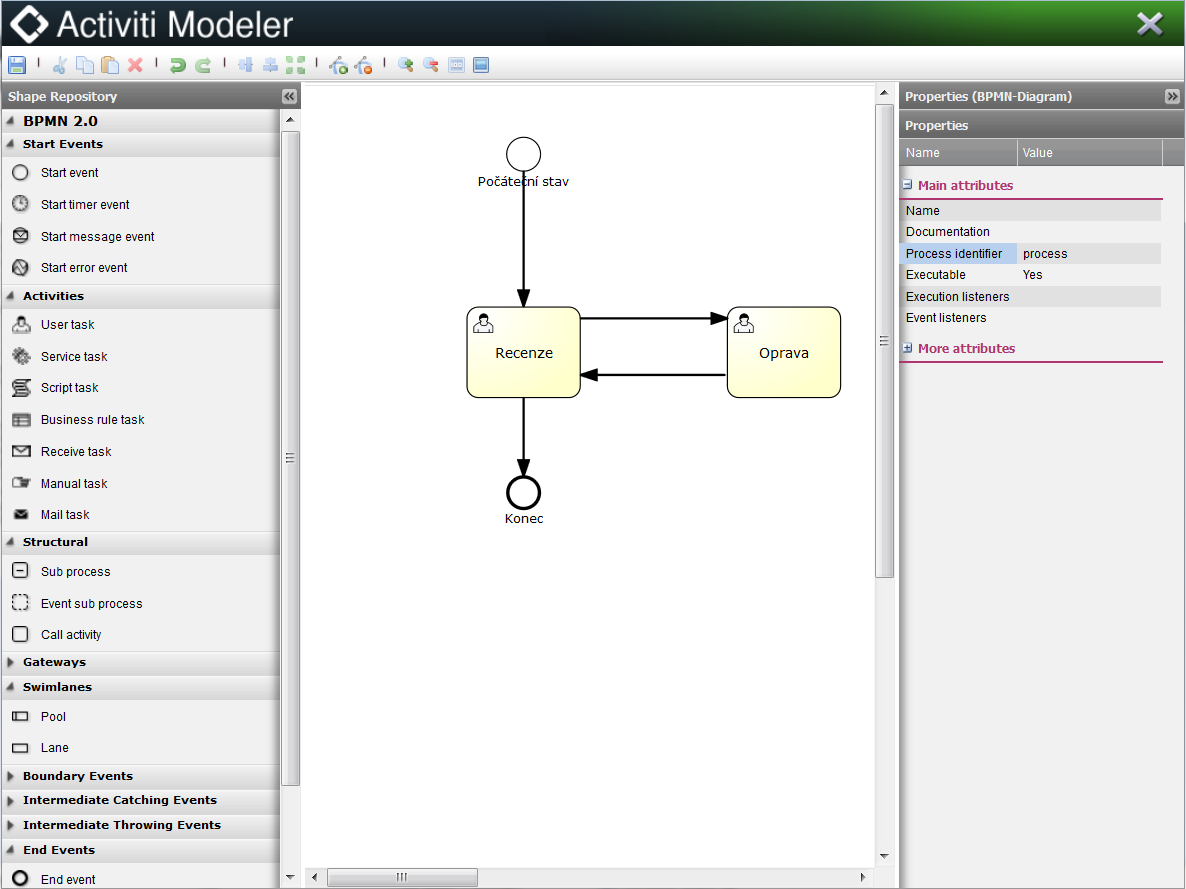
\includegraphics[width=330px]{images/activiti_modeler.png}
\caption{Activiti modeler}
\label{fig:activiti_modeler}
\end{figure}

Celá aplikace se skládá ze čtyř základních panelů. V prvním horní vodorovném panelu jsou uloženy všechny tlačítka, které reprezentují všechny akce, které je možné při modelování využít. Panel vlevo slouží jako paleta dostupných BPMN elementů. Na plátno, což je prostřední panel, se vkládají pomocí metody táhni a pusť. Poslední panel, umístěný vpravo, slouží pro úpravy vlastností jednotlivých entit či vlastností celého workflow.

\section{Kaleo}
Portál Liferay od verze 6.0 obsahuje workflow systém Kaleo, který je vyvíjen společně s portálem. Umožňuje uživatelům definovat jednoduché i složitější procesy, nasadit je a spravovat pomocí rozhraní v portálu. Tyto procesy mohou pracovat s uživateli, skupinami a rolemi z portálu, aniž by bylo nutné napsat jediný řádek zdrojového kódu. Tyto definice je ale nutné vkládat v~podobě XML dokumentů s definovanou strukturou. 

Ve verzi portálu Liferay EE je k dispozici pro návrh workflow definic Kaleo Designer. Je přímo součástí portálu a je dostupný z ovládacího panelu. V něm je možné vytvářet workflow definice pomocí grafického rozhraní a~následně je vkládat do portálu a dále je využívat.

Kaleo Designer je možné rozdělit na dvě hlavní obrazovky. Na první je zobrazen seznam dostupných workflow v portálu. Druhá obsahuje samotné grafické rozhraní pro tvorbu a úpravu definic. V dalším popisu se zaměřím pouze na grafické rozhraní, jehož detail můžeme vidět na obrázku \ref{fig:kaleo_designer}.

\begin{figure}[h]
\centering
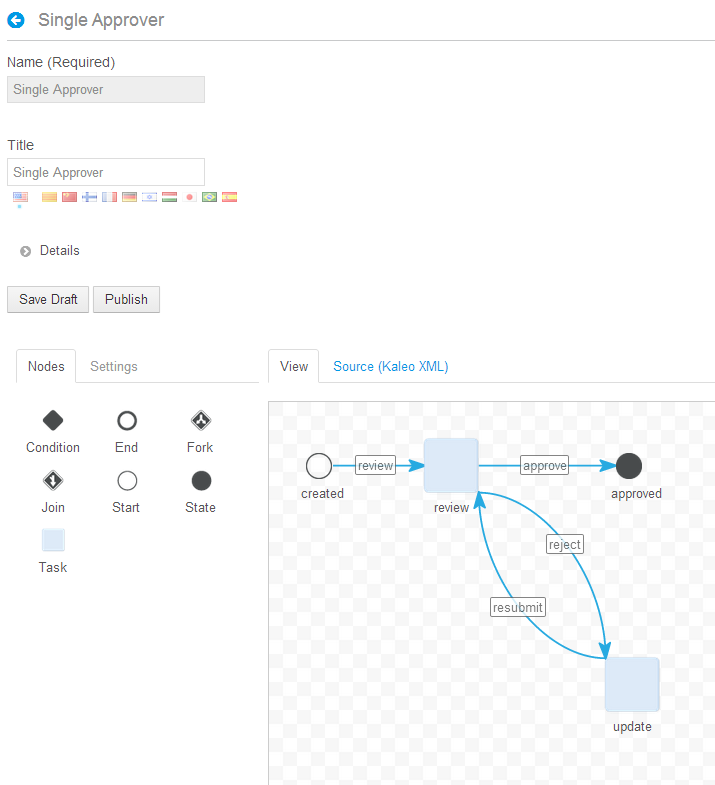
\includegraphics[width=300px]{images/kaleo_designer_detail.png}
\caption{Kaleo Designer detail}
\label{fig:kaleo_designer}
\end{figure}

Kaleo workflow designer se také skládá ze tří základních panelů. V horním panelu jsou zobrazeny základní informace o workflow, tedy hlavně jméno, popis a také verzi návrhu. Dále jsou zde také tlačítka pro uložení návrhu a~vložení workflow definice do portálu.

Další panel umístěný na levé straně obrazovky slouží buď jako paleta dostupných elementů pro tvorbu workflow nebo po vybrání některého elementu se v tomto panelu zobrazují podrobnosti o daném elementu. Ty je možné měnit pomocí kliknutí na vybranou vlastnost, po kterém se zobrazí vyskakovací okno, které obsahuje formulář pro změnu. Tyto formuláře mohou ovšem také obsahovat další odkazy pro změnu dalších vlastností a pak se vyskakovací okna řetězí přes sebe.  Takto zobrazené formuláře pak nemusí působit z uživatelského hlediska přívětivě a je celkem jednoduché ztratit přehled o prováděných změnách. Ukázku takovéto nepřehledné situace můžeme vidět na obrázku \ref{fig:kaleo_designer_popup}.  

V pravé části obrazovky je umístěn přepínací panel obsahující v jedné záložce vlastní plátno s grafickými editorem a v druhé záložce pak textový editor zobrazující výsledný XML dokument právě vytvářené workflow definice. Na obou místech je možné workflow definici měnit.

\begin{figure}[htp]
\centering
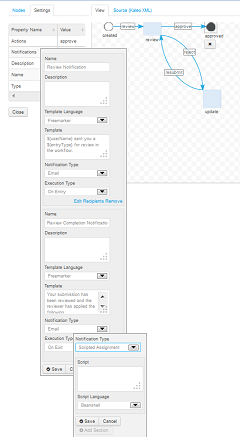
\includegraphics[width=240px, height=400px]{images/kaleo_designer_popup.png}
\caption{Řetězení vyskakovacích oken}
\label{fig:kaleo_designer_popup}
\end{figure}

\section{Požadavky na vytvářenou aplikaci}
Grafický editor pro tvorbu je velice speciální aplikace a při analýze požadavků jsem zjistil, že tento produkt má pouze jeden diagram užití. Hlavně z~tohoto důvodu jsem zvolil analýzu v podobě seznamu skupin požadavků. Takovýto způsob zápisu je také bližší zákazníkům, kterým bude následně tento produkt nabízen. 

\begin{center}
\begin{longtable}{|p{5.5cm}|p{5.5cm}|}
\caption{Seznam skupin požadavků}\\
\hline
\textbf{Požadavek} & \textbf{Návrh řešení}  \\
\hline
\endfirsthead
\multicolumn{2}{c}%
{\tablename\ \thetable\ -- \textit{Pokračování z předchozí strany}} \\
\hline
\textbf{Požadavek} & \textbf{Návrh řešení}  \\
\hline
\endhead
\hline \multicolumn{2}{r}{\textit{Pokračování na další straně}} \\
\endfoot
\hline
\endlastfoot
\hline Kompatibilita s workflow systémem používaným v Liferay CE. & Výsledné XML schéma bude odpovídat požadovanému schématu workflow systémem Kaleo.  \\
\hline Aplikace umožní vytvářet a vkládát nové workflow definice. Také umožní načítat již vložené definice v portálu.  & Aplikace bude napojena skrz portálové API Liferay k portálu. \\
\hline Aplikace umožní exportovat výsledné definice ve formátu XML.  & Bude možné exportovat vytvářené workflow definice do souboru ve formátu XML. \\
\hline  Aplikace bude v portálu přístupný pouze pro administrátory. & Editor bude umístěn v ovládacím panelu portálu v sekci konfigurace. \\
\hline Aplikace by být přehledná a jednoduše použitelná.  & Bude omezeno použití vyskakovacích oken, které aplikace tohoto typu znepřehledňují. \\
\hline V editoru bude vytvářet i rozsáhlejší workflow definice.  & Editor bude umožňovat nastavit libovolnou velikost plátna. \\
\hline Uživatel bude mít možnost zkontrolovat správnost vytvářené workflow definice.  &  Editor bude umožňovat validaci vytvářené workflow definice. \\
\hline Editor umožní uživateli vracet zpět provedené úpravy.  & Editor bude podporovat funkcionalitu zpět / vpřed. \\
\hline Editor bude pracovat v základní notaci BPMN.  & Tento požadavek je omezen vlastnostmi workflow systému Kaleo, jenž umožňuje využít pouze některé prvky. \\
\hline Editor bude umožňovat tvořit a~upravovat skripty k akcím u jednotlivých elementů. & K těmto účelům bude k dispozici webový editor. \\
\hline K tvorbě skriptů bude mít uživatel k dispozici předpřipravené některé nejpoužívanější funkce.  &   Bude k dispozici seznam vložitelných funkcí v jednom zvoleném skriptovacím jazyku. \\
\hline Výsledná aplikace by měla grafickým rozhraním zapadat do prostředí Liferay Portálu. & Pro tvorbu grafického rozhraní budou využity technologie, které jsou použity pro tvorbu grafického rozhraní portálu.\\
\hline Kde to bude možné, bude ve formulářích dostupné automatické doplňování uživatelů z portálu. & Bude vytvořeno napojení na portálovou databázi uživatelů a rolí.

\end{longtable}
\end{center}



\chapter{Realizace}
Aplikace není tvořena klasickou třívrstvou architekturou, protože není potřeba řešit perzistenci dat přímo v aplikaci. Výsledná workflow definice se buď vkládá přímo do portálu skrze portálové api nebo je možné výsledný XML soubor exportovat z aplikace. Proto se v následující části zaměřím hlavně na popis prezentační vrstvy a využití portálového api.

\section{Portletové MVC rámce}
Ve druhé kapitole byl představen životní cyklus portletu a hlavní koncepty vývoje portletů v Javě. Při vývoji podle portletové specifikace se portlet vytváří rozšířením třídy  \verb|GenericPortlet| a pomocí action a render metod, které obsahují navigační a validační logiku a zároveň se starají o zpracování akcí a generování obsahu. S přibývajícím množstvím funkcí se pak tato třída stává nepřehlednou a špatně udržovatelnou. Tento problém je možné řešit tím, že se rozdělí zodpovědnosti za zpracování požadavků do více specificky zaměřených komponent pomocí některého portletového rámce.

Portletové nebo webové rámce v sobě implementují osvědčené postupy a~vzory pro zjednodušení vývoje. Pro vývoj portletů lze využít i ne přímo portletových rámců, například Struts nebo JSF, ale v takovémto případě je nutné použít takzvané portletové mosty, které řeší rozdíly mezi servletovým a portálovým životním cyklem. Toto řešení ale v sobě obsahuje vícefázový životní cyklus portletů a někdy to znesnadňuje využití plných možností portletové technologie. Portletový rámec navržený přímo pro vývoj portletů je rámec Spring MVC Portlet, který byl zvolen také pro vývoj této aplikace. Tento portletový rámec byl zvolen zejména proto, že je standardně používaný ve firmě IBA CZ, pro kterou je tato práce řešena v rámci Sdružení průmyslových partnerů Fakulty informatiky.

\subsection*{Spring Portlet MVC}
Rámec Spring Portlet MVC je založen na stejných konceptech, třídách a rozhraní jako Spring Web MVC framework \cite{spring-web-mvc}. Spring Portlet MVC je navržen pouze pro vývoj portletů a je možné pomocí něj vyvíjet portlety, které splňují portletové standardy JSR-168 i JSR-286. Také implementuje klasickou architekturu MVC. Ta se skládá z následujících částí. \cite{mvc} 

\begin{itemize}
\item Model (model) - je to doménově specifická reprezentace informací s~nimiž aplikace pracuje.
\item View (pohled) - převádí data reprezentovaná modelem do vhodné podoby  k prezentaci uživateli.
\item Controller (řadič) - reaguje na události a zajišťuje změny v modelu a~pohledu.
\end{itemize}

Nejdůležitější roli v portletu má třída \verb|DispatcherPortlet|, která obstarává všechny příchozí požadavky, pro které volí vhodný řadič na zpracování požadavku. Každá instance dispečeru si udržuje vlastní aplikační kontext.


\section{Alloy UI framework}
Alloy je UI meta framework, který poskytuje konzistentní a jednoduché API pro vytváření webových aplikací na třech úrovní prohlížeče: struktura, styl a chování. Je založených na moderních technologiích CSS3, HTML5 a javascriptovém frameworku YUI3. \cite{alloy} V Liferay Portal od verze 6 nahradil tento framework dříve používaný jQuery a je na něm postaveno celé grafické rozhraní portálu Liferay.

\begin{figure}[htp]
\centering
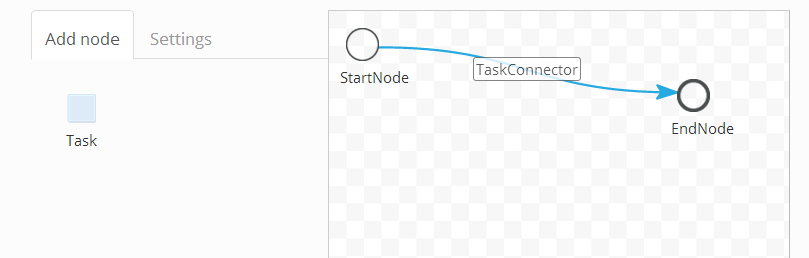
\includegraphics[width=340px, height=100px]{images/diagram_builder.png}
\caption{Alloy UI Diagram Builder komponenta}
\label{fig:diagram_builder}
\end{figure}

Pro využití tohoto frameworku jsem se rozhodl z několika důvodů. Liferay Portal tento framework využívá pro tvorbu grafického rozhraní celého portálu a je proto již standardní součástí portálu, což jeho využití zjednodušuje. Jeho použitím také dosáhnu stejného vzhledu aplikace jako je vzhled portálu, což je také jedním z požadavků kladených na tuto aplikaci. Dalším důvodem bylo, že Alloy UI poskytuje mnoho připravených komponent, které je možno využít. Některé podstatné popíši blíže. 

Z pohledu této práce je nejdůležitější komponentou \textbf{Diagram Builder}, obrázek  \ref{fig:diagram_builder}. Pro potřeby aplikace musela být tato komponenta rozšířena a~upravena. Na ukázce zdrojového kódu \ref{code:diagram_builder} je vidět základní postup, jakým se rozšiřují komponenty z frameworku Alloy UI.

\begin{lstlisting}[language=JavaScript, caption = Rozšíření komponenty Diagram Builder , label = code:diagram_builder]
AUI.add('my-diagram-builder', function(A, NAME) {
   var MyDiagramBuilder = A.Component
      .create({
         NAME : DIAGRAM_NAME,
         EXTENDS : A.DiagramBuilder,

          prototype : {
             select : function(diagramNode) {
             }
          }
   });
   A.MyDiagramBuilder = MyDiagramBuilder;

}, '2.0.0', {
	requires : [ ],
});

\end{lstlisting}

V části \verb|EXTENDS : A.DiagramBuilder| je definováno, jaká komponenta je rozšiřována. V bloku \verb|prototype| jsou umístěny přepisované či nově definované funkce a právě v této části bylo provedeno nejvíce změn. V části \verb|A.MyDiagramBuilder = MyDiagramBuilder| je nová komponenta přidána do frameworku Allyou UI a je možné ji možné používat v aplikaci. Vzhled komponenty je možné ovlivnit přepsáním daných třídy v css pravidlech. Celou komponentu po  provedených úpravách můžeme vidět na obrázku  \ref{fig:diagram_builder_uprav}.

\begin{figure}[htp]
\centering

\includegraphics[width=340px]{images/diagram_builder_uprav.png}
\caption{Alloy UI komponenta Diagram Builder po úpravách}
\label{fig:diagram_builder_uprav}
\end{figure}

Další komponentou využitou v aplikaci je \textbf{Ace editor}. Ta se využívá pro psaní vlastních skriptů pro jednotlivé akce přiřazované jednotlivým uzlům, či definování skriptu pro podmínky při tvorbě definice workflow. Pro psaní těchto skriptů je možné využít různé skriptovací jazyky. Tuto komponentu k~těmto účelům nebylo nutné nijak rozšiřovat. Je však využito možnosti nastavit tzv. mód editoru v závislosti na zvoleném skriptovacím jazyku, což pak zajišťuje barevné zvýraznění syntaxe daného jazyka. Dále byla ještě přidána při tvorbě skriptů možnost vkládat některé definové často používané funkce při tvorbě workflow definic v portálu Liferay. Pro účely aplikace bylo vytvořeno několik funkcí v jazyku Groovy. Uživatel má také možnost přidávat své vlastní funkce. Na souborovém disku vytvoří adresář se jménem scripts a v něm další adresář se názvem podle scriptovacího jazyka, u kterého mají být funkce zobrazovány. Do tohoto adresáře jsou pak vkládány scripty s funkcemi. Cestu k tomuto adresáři pak musí zadefinovat v konfiguračním souboru portálu Liferay \verb|portal-ext.properties| takto:

\begin{lstlisting}[language=Java , caption = Definovaná cesta ke skriptům , label =code:cesta] 
cz.muni.fi.mtlacbaba.designer.scripts="skripty"
\end{lstlisting} 


Pak jsou také tyto funkce načteny a k dispozici při tvorbě workflow definic. Výsledný vzhled editoru na úpravu skriptů je vidět na obrázku \ref{fig:ace_editor}.
 
\begin{figure}[htp]
\centering
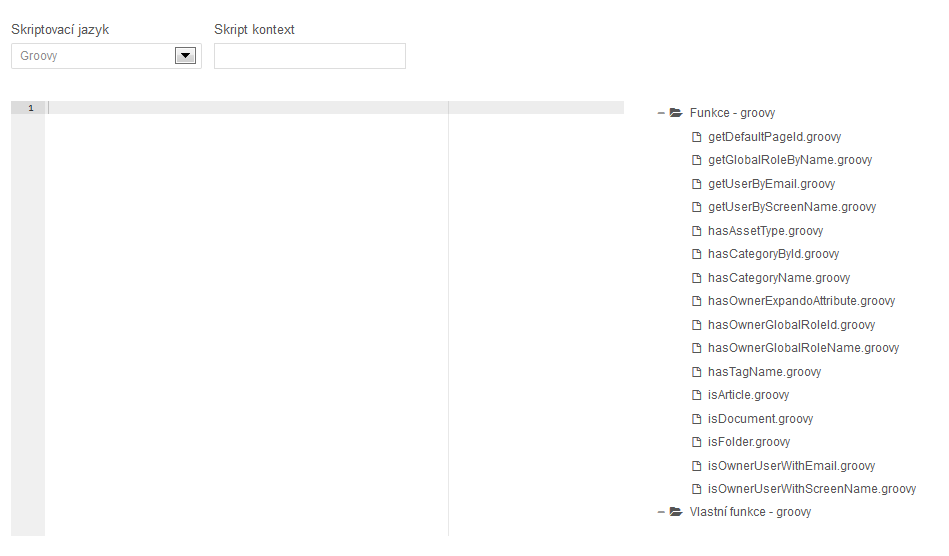
\includegraphics[width=340px]{images/ace_editor.png}
\caption{Ace editor použitý v aplikaci}
\label{fig:ace_editor}
\end{figure}

Pro validaci formulářů byla využita další komponenta, \textbf{Form Validator}. Je použita pro veškeré validace vstupů od uživatele ve všech formulářích.

\begin{lstlisting}[language=JavaScript , caption = Použítí komponenty Form Validator , label = code:validator]
var actionValidator = new A.FormValidator({
   boundingBox: '#action-form', 
   rules: {
      name: {required: true},
      priority: {digits:true}
   }
});
\end{lstlisting}

V ukázce \ref{code:validator} můžeme vidět použití komponenty. V ní \verb|rules| představuje pole omenzení pro jednotlivé pole formuláře pro zadání nové akce. Pole \verb|name| je povinné a pole \verb|priority| může obsahovat pouze číslice. Validator je uložen do proměnné \verb|actionValidator| a navázán na formulář s id \verb|action-form|. Nakonec při vložení nesprávných vstupů může validator vypadat třeba jako na obrázku \ref{fig:validator}.

\begin{figure}[htp]
\centering
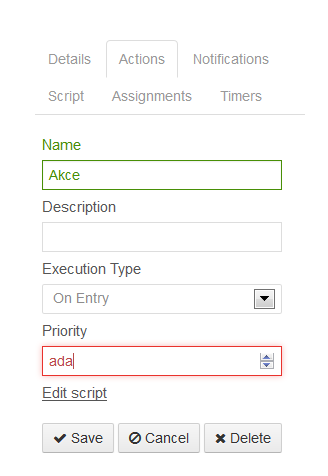
\includegraphics{images/validator.png}
\caption{Form Validator}
\label{fig:validator}
\end{figure}

Další použitou komponentu  je Autocomplete. V ukázce \ref{code:autocomplete} vidíme použití této komponenty. V proměnné \verb|data| jsou data použitá pro našeptávání, která jsou posílány ze serverové části aplikace a tam jsou získáváná pomocí portálového API, které bude blíže vysvětleno v kapitole \ref{sec:portal_api}. V části \verb|resultHighlighter: 'phraseMatch'| se nastavují pravidla pro zvýrazňování fráze při výběru, v tomto případě se zvýrazňuje celá fráze. V části \verb|resultFilters: 'charMatch'| se  nastavují pravidla pro vyhledávání v nápovědě. Zde je nastaveno  vyhledávání podle zadaných znaků, které slova obsahují i v různém pořadí. Použití v aplikaci vypadá například jako na obrázku \ref{fig:autocomplete}.

\begin{lstlisting}[language=JavaScript, float =h , caption = Použítí komponenty autocomplete , label = code:autocomplete ]
var data = ["default@liferay.com-10161", 
                  "test@liferay.com-test"]

A.one('#role').plug(A.Plugin.AutoComplete, {
	resultHighlighter: 'phraseMatch', 
     resultFilters: 'charMatch',
	source: data
});
\end{lstlisting}



\begin{figure}[htp]
\centering
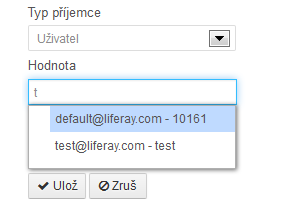
\includegraphics{images/autocomplete.png}
\caption{Autocomplete}
\label{fig:autocomplete}
\end{figure}


\section{JAXB}
K ukládání worfklow definice je využíván dokument ve formátu XML a~struktura XML dokumentu používaného workflow systémem Kaleo je definovaná XML schématem, označovaném jako XML Schema Definition (XSD). Je to XML dokument s pevnou strukturou obsahující omezující podmínky na strukturu a obsah XML dokumentu. Proto je možné využít klasické nástroje pro práci s XML a jedno z možných využití je generování anotovaných Java tříd popisující XML dokumenty vyhovující danému XML schématu. 

K tomuto účelu jsem zvolil nástroj JAXB, jenž umožňuje tvořit návaznosti mezi Java objekty a XML schématem, díky nimž je pak možno zpracovávat XML dokumenty. Tento nástroj je založený na anotacích a poskytuje rozhraní pro serializaci a deserializaci Java objektů do/z XML dokumentů podle daných anotací. Navíc také poskytuje vyšší úroveň abstrakce než SAX \footnote{SAX je zkratka pro Simple API for XML} či DOM \footnote{DOM je zkratka pro Document Object Model} a~je součástí JDK.

Pro vygenerování sady tříd jazyka Java na základě daného schématu jsem využil kompilátor vazeb (xjc), jenž je také součástí JDK. Takto byly anotované třídy sloužící pro konvertování XML dokumentů do stromů objektů a~zpět. Ukázku takto anotované třídy můžeme vidět zde \ref{code:jaxb}.

\begin{lstlisting}[language=Java, float =h , caption = Java třída s JAXB anotacemi , label = code:jaxb ]
@XmlAccessorType(XmlAccessType.FIELD)
@XmlType(name = "abstract-workflow-node-complex-type", 
propOrder = {
    "name",
    "description",
    "metadata"
})
@XmlSeeAlso({
    Task.class,
    ActionTimerWorkflowNodeComplexType.class
})
public abstract class AbstractWorkflowNodeComplexType{

    @XmlElement(required = true)
    protected String name;
    protected String description;
    protected String metadata;
//upraveno
}

\end{lstlisting}

Z takto anotovaných tříd je vytvořen strom objektů, který reprezentuje obsah a strukturu XML dokumentu. Pomocí těchto tříd je možné upravovat reprezentaci dokumentu a nakonec je tento strom převeden na XML dokument. S tímto je spojena první fáze validace workflow definice, jelikož se tímto kontroluje, zda odpovídá zadanému schématu. Tímto je pouze zaručené, že workflow definice obsahuje validní objekty, ale ještě není zaručeno, že workflow je validní jako celek. Úplná validace se provádí skrze portálové~API.



\section{Liferay Portal API} 
\label{sec:portal_api}
Liferay Portal API\footnote{Zkratka pro Application Programing Interaface označuje rozhraní pro programování aplikací.} poskytuje vývojářům přístup ke zdrojům v portálu. Mezi tyto zdroje například patří uživatelé, role, články, dokumenty, workflow a další. S těmito zdroji je možné pracovat skrze servisní třídy poskytující metody pro manipulaci s nimi.

V některých formulářích bylo implementováno našeptání uživatelů a rolí existujících v portálu. K tomu účelu byly využity následující statické servisní třídy: 
\begin{itemize}
\item pro uživatele  (\verb|UserLocalServiceUtil|),
\item pro role (\verb|RoleLocalServiceUtil|).
\end{itemize}
V ukázce \ref{code:users} vidíme načtení všech existujících uživatelů z portálu.

\begin{lstlisting}[language=Java, float =h , caption = Načtení uživatelů z portálu , label = code:users ]
List<User> users = UserLocalServiceUtil.getUsers(-1, -1));
\end{lstlisting}

Třída \verb|WorkflowDefinitionManagerUtil| byla využita pro načítání, vkládání a validaci workflow definic. Ukázka \ref{code:workflow} ukazuje proces validace workflow. Proces validace v tomto případě probíhá následovně. Vytvořené workflow se validuje pomocí metody \verb|validateWorkflowDefinition|. Pokud je workflow validní, tak metoda úspěšně skončí, pokud ovšem workflow validní není, tak je vyhozena vyjímka, která obsahuje důvod selhání validaci. Tato vyjímka je aplikací zachycena a důvod selhání je vrácen uživateli v podobě chybové hlášky jak je vidět na obrázku \ref{fig:error}

\begin{lstlisting}[language=Java, float =h , caption = Validace workflow pomocí portálového API , label = code:workflow ]
try {
WorkflowDefinitionManagerUtil.
validateWorkflowDefinition(xml.getBytes("utf-8"));
        } catch (WorkflowException e) {
        //zpracovani vyjimky
        }
}
\end{lstlisting}


\begin{figure}[htp]
\centering
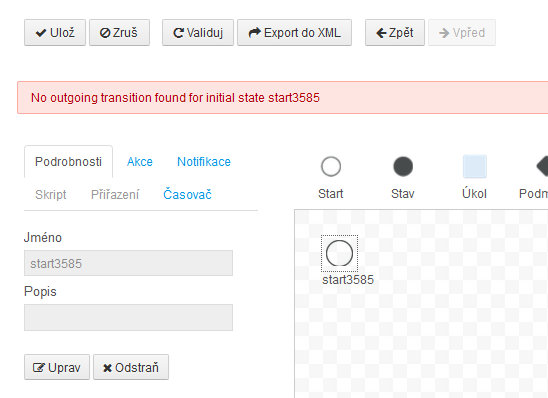
\includegraphics[width=340px]{images/error_message.png}
\caption{Chybová hláška při validaci worklow}
\label{fig:error}
\end{figure}





\chapter{Testování aplikace}
Testováním je možné nazvat jakoukoliv aktivitu, která odhalí, že chování programu porušuje specifikaci. Nejčastěji bývá na testování nahlíženo jako na disciplínu, jejímž úkolem je ověřování kvality. Příkladem může být definice od Kanera \cite{kaner}: Softwarové testování je empirický technický výzkum kvality testovaného produktu nebo služby, prováděný za účelem poskytnutí těchto informací lidem, kterí mají zájem na dané věci. Na pojem kvalita produktu v tomto případě může být nahlíženo tak, že produkt má splnit požadavky určité potřeby, která stojí za jeho vznikem. Tedy kvalitní software je takový, který tyto potřeby uspokojuje.

Množina využitelných testů je velmi široká a proto je vždy nutné určit, jaké druhy testů budou použity, kdy a jak budou aplikovány. Webové aplikace patří do speciální skupiny softwaru a proto se zde používají určité druhy testování a ty je možné rozdělit do kategorií \cite{web-test}:  funkční testování, výkonnostní testování, testování použitelnosti, testování serverového rozhraní, testování kompatibility a testování bezpečnosti.

\section{Zvolené druhy testů}
Pro účely této aplikace jsem jako nejvhodnější zvolil funkční testování v~kombinaci s testováním kompatability.

\subsection*{Funkční testování}
Je to postup, kdy je ověřováno správné fungování aplikace nebo její části podle předem definovaného nebo očekávaného chování. Aplikace se při tomto testu prochází z pohledu uživatele a je tedy kontrolováno, zda reakce na uživatelovy akce a vstupy jsou správné a jestli aplikace podává správné výstupní informace a výsledky.

Zde je možné zahrnout kontrolu správnosti odkazování, ověřování funkčnosti formulářových prvků včetně validace vstupů a reakcí na chybný vstup. Mezi další patří také správná funkčnost JavaScript nebo AJAX částí aplikace.

\subsection*{Testování kompatability}
Protože existují různé platformy spolu s rozmanitými prohlížeči, kde mohou být webové aplikace spouštěny, je testování kompatability velmi důležité. Je tedy vždy vhodné otestovat aplikaci na nejběžnějších kombinacích systémů, aby se tak zajistila správná funkčnost aplikace pro co nejširší okruh uživatelů.

\section{Příprava a průběh testů}
Aplikace workflow editor je určena pro tvorbu workflow definic v portálu Liferay. Jejím jediným uživatelem je administrátor portálu.Testování probíhalo podle předem určených určených testových scénářů na různých prostředí a~v~různých webových prohlížečích. Testové scénáře (TS) pokrývají všechny důležité funkce editoru. 
\begin{itemize}
\item TS-01 Vytvoření nového workflow.
\item TS-02 Změna již vloženého workflow.
\item TS-03 Exportování workflow do dokumentu ve formátu XML.
\item TS-04 Přidání nového uzlu.
\item TS-05 Přidání akce k uzlu.
\item TS-06 Úprava akce u uzlu.
\item TS-07 Přidání oznámení k uzlu.
\item TS-08 Úprava oznámení u akce.
\item TS-09 U uzlu typu podmínka úprava scriptu.
\item TS-10 U uzlu typu úloha úprava přiřazení.
\item TS-11 Přidání časovače u uzlu.
\item TS-12 Úprava časovače u uzlu.
\item TS-13 Validace workflow.
\end{itemize}
Následuje úkazka vybraného testového scénaře.


\subsection*{Testový scénář - TS-02 Změna již vloženého workflow}
 

\textbf{Vstupní podmínky:} Uživatel je v roli Administrátora (má tedy přístup do kontrolního panelu), je přihlášený v portálu a nachází se v sekci kontrolní panel. Uživatel již vytvořil workflow definici a vložil ji do portálu na základě TS--01~Vytvoření nového workflow.

\textbf{Scénář:}
\begin{enumerate}
\item Přechod na stránku s workflow editorem
\item Kliknutí na odkaz "Edit" na řádku workflow vytvořeného na základě Vytvoření nového workflow
\item Přidání nového stavu kliknutím na ikonu "Nový stav" (vizuální podoba - kruh)
\item Kliknutím do kreslící plochy (tímto se umístí nový stav)
\item Kliknutím na nově vytvořený stav 
\item Pak táhnutím nad cílový stav a kliknutím na něj se vytvoří nová vazba
\item Kliknutí na tlačítko "Uložit" pro uložení pozměněného workflow

\end{enumerate}


\section{Vyhodnocení testů}
Testové scénáře byly prováděny průběžně ihned po implementaci jednotlivých částí na prostředí Windows 7 a v prohlížeči Firefox. Problémy v nich nalezené byly ihned opravovány a nebyly nijak dokumentovány.

Po dokončení celé aplikace jsem přistoupil k provedení všech testových scénářů v prostředí s  operačním systémem Windows 7 (W7) a zde jsem zvolil prohlížeče Internet Explorer (IE) ve verzích 9,11 a prohlížeče Google Chrome (Chrome) ve verzi 34 a Firefox (FF) ve verzi 29. Jako druhé testovací prostředí jsem zvolil linuxovou distribuci Ubuntu 14.04 LTS a zde byly zvoleny prohlížeče Google Chrome ve verzi 34 a Firefox ve verzi 28.

Bylo tedy prováděno 12 testových scénářů na celkem na 6 různých prostředí. V tabulce  \ref{tab:chyby} jsou uvedeny všechny nalezené chyby při provádění scénářů. V první sloupci je scénář a prostředí, pokud se chyba vyskytla pouze ve specifickém prostředí a v druhém sloupci je popis chyby.

\begin{center}
\begin{longtable}{|p{3cm}|p{8cm}|}
\caption{Vyhodnocení testových scénářů}
\label{tab:chyby}\\

\hline
\textbf{Scénář} & \textbf{Nalezené chyby}  \\
\hline
\endfirsthead
\multicolumn{2}{c}%
{\tablename\ \thetable\ -- \textit{Pokračování z předchozí strany}} \\
\hline
\textbf{Scénář} & \textbf{Nalezené chyby}  \\
\hline
\endhead
\hline \multicolumn{2}{r}{\textit{Pokračování na další straně}} \\
\endfoot
\hline
\endlastfoot
\hline TS-01 W7 - IE & Šedý čtvereček nad výběrem elementům je chybně navíc.\\
\hline TS-03 & Je možné exportovat i nevalidní workflow definici.\\
\hline TS-05 & Vypsání chybové hlášky pohne zbytkem formuláře směrem dolů. Týká se všech formulářů v aplikaci.\\
\hline TS-05 & Validator se neresetuje po zrušení formuláře. Týká se všech formulářů v~aplikaci.\\
\hline TS-13 & Zobrazení chybové hlášky posune celou aplikaci dolů, po zmizení hlášky se opět celá aplikace posune zpět.\\

\end{longtable}
\end{center}

Nalezené chyby byly opraveny a zopakování testových scénářů ověřilo odstranění chyb.

\chapter{Dokumentace}
V této kapitole bude popsána vytvořená uživatelská dokumentace pro aplikaci Workflow Editor. Celá dokumentace je vytvořena v systému confluence firmy IBA CZ a není dostupná z veřejné sítě. Proto je zde pouze struktura dokumentace a poté je připojena ukázka.

\begin{itemize}
\item Úvod a základní popis aplikace
\item Vytvoření či načtení existujícího workflow
\item Úpravení záklaldní vlastností workflow
\item Vytvoření nového uzlu ve workflow a úpravy základních vlastností
\item Vytvoření a úpravy vazby mezi uzly
\item Vytvoření a úpravy akce u zvoleného uzlu
\item Vytvoření a úpravy oznámení u zvoleného uzlu
\item Vytvoření a úpravy přiřazení u uzlu typu úloha
\item Vytvoření a úpravy skriptu u uzlu typu podmínka
\item Vytvoření a úpravy časovače u uzlu
\item Validace, uložení a export workflow
\end{itemize}

Na přiloženém obrázku \ref{fig:dokumentace} můžeme vidět část dokumentace nacházející na v systému confluence firmy IBA CZ.

\begin{figure}[htp]
\centering
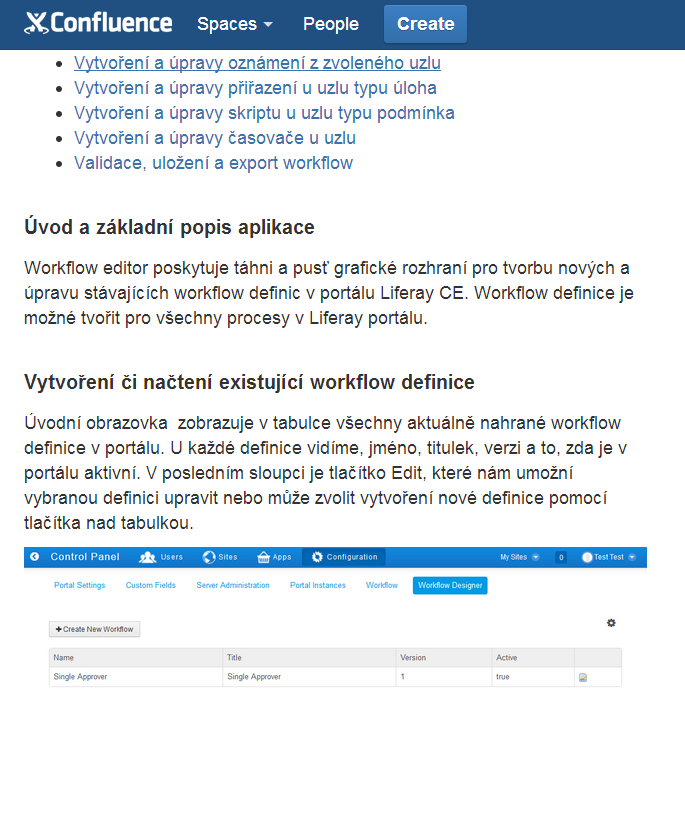
\includegraphics[width=340px]{images/screen_confluence.png}
\caption{Ukázka z dokumentace}
\label{fig:dokumentace}
\end{figure}

\chapter{Závěr}
Cílem této práce bylo seznámit se s problematikou podnikových portálů a~tvorbou portletových aplikací. Praktickým výstupem práce bylo navrhnout a implementovat grafický workflow editor pro standardantí workflow systém v portálu Liferay CE.

Cíle práce se podařilo splnit. Úvodní část práce poskytuje základní orientaci v oblasti podnikových portálů i čtenáři, který s nimi nemá předchozí zkušenost. Byly mu představeny výhody při nasazení portálu v podnikovém prostředí, kdy portál slouží jako integrační platforma pro přístup k aplikacím a různým zdrojům. Byla představena dostupná portálová řešení a poté se práce blíže věnovala portálu Liferay, pro který je vytvářena aplikace. Pak byl čtenář seznám s vývojem portletů pomocí portletových specifikací JSR-168 a JSR-286. Byl představen životní cyklus portletové aplikace, architektura portálu a další specifika vývoje portletů. Dále byl čtenář seznámen s oblastí worklow systémů, jejich dělení a obecným modelem workflow. Také mu byla představena notace BPMN používaná pro modelování podnikových procesů.

Bylo provedeno srovnání s podobnými řešeními pro jiné workflow systémy a následně byla provedena analýza požadavků, jejímž výsledkem byl seznam požadavků kladených na nový workflow editor pro systém Kaleo. Navržená aplikace byla implementována pomocí moderních technologií platformy Java EE. Prezentační vrstva využívá rámec Spring portlet MVC společně s frameworkem Alloy UI. Část práce byla věnována problematice práce s dokumenty ve formátu XML v jazyku Java. Při vytváření aplikace byly průběžně procházeny testové scénáře podle toho, jaké funkce byly aktuálně implementovány. Nakonec byly provedeny všechny vytvořené testové scénáře na různých prostředích.

Hlavní přínos pro mne vidím v seznámení se s oblastí podnikových portálů a v získání zkušeností s vývojem systému pomocí technologií platformy Java EE. Práce byla řešena v rámci průmyslového partnerství Fakulty informatiky se společností IBA CZ.




%\printindex


\begin{thebibliography}{0}


\bibitem{gala}
GÁLA, L. \textit{Podniková informatika}. 1. vyd. Praha: Grada, 2006. 

\bibitem{jsr-286}
HEPPER, S. \textit{JavaTM Portlet Specification Version 2.0}, [online] 2008 [cit. 2014-03-27]. Dostupné z \url{http://www.jcp.org/en/jsr/detail?id=286}.

\bibitem{cech}
ČECH, P. \textit {Přínos podnikových portálů pro management znalostí}, in Internet a konkurenceschopnost, Zlín, 2004.

\bibitem{enterprise-portal}
Enterprise portal. \textit{Wikipedia: the free encyclopedia} [online]. San Francisco (CA): Wikipedia Foundation,2011-, naposledy upraveno 7.2.2014 [cit. 2014-03-27]. Dostupné z \url{http://en.wikipedia.org/wiki/Enterprise_portal} .

\bibitem{developer-guide}
LIFERAY. Liferay Portal 6.2 Developer's Guide. In: \textit{Liferay.com} [online].  [cit. 2014-04-02]. Dostupné z \url{http://www.liferay.com/documentation/liferay-portal/6.2/development}

\bibitem{liferay-features}
LIFERAY. Portal Features. In: \textit{Liferay.com} [online]. [cit. 2014-04-02]. Dostupné z \url{http://www.liferay.com/products/liferay-portal/features/portal}

\bibitem{portlets-in-action}
ASHISH, S. \textit{Portlets in Action}, Shelter Island, NY: Manning Publications, 2011.

\bibitem{wfmc}
Terminology \& Glossary. \textit{Workflow Management Coalition} [online]. [cit. 2014-04-14]. Dostupné z \url{http://www.wfmc.org/standards/docs/TC-1011_term_glossary_v3.pdf} 

\bibitem{workflow}
CARDA, A., KUNSTOVÁ, R. \textit {Workflow : Nástroj manažera pro řízení podnikových procesů}. 2. vyd. Praha: Grada Publishing, 2003.

\bibitem{bpmn}
OBJECT MANAGEMENT GROUP. \textit{Business Process Model and Notation (BPMN)} [online]. 2011 [cit. 2014-04-23]. Dostupné z \url{http://www.omg.org/spec/BPMN/2.0/} 

\bibitem{activiti}
RADEMAKERS, Tijs. \textit{Activiti in action}. Shelter Island, NY: Manning Publications, 2012.

\bibitem{spring-web-mvc}
Web MVC framework. \textit{Spring Framework Reference Documentation} [online]. [cit. 2014-05-04]. Dostupné z \url{http://static.springsource.org/spring/docs/current/
spring-framework-reference/html/mvc.html} 

\bibitem{mvc}
Model-view-controller. \textit{Wikipedia: the free encyclopedia} [online]. San Francisco (CA): Wikipedia Foundation,2011-, naposledy upraveno 23.1.2014 [cit. 2014-03-27]. Dostupné z \url{http://en.wikipedia.org/wiki/Model-view-controller} .

\bibitem{alloy}
LIFERAY. \textit{About} [online]. [cit. 2014-04-06]. Dostupné z \url{http://alloyui.com/about/}

\bibitem{kaner}
ABRAN, A., MOORE, J.W. \textit{Guide to the Software Engineering Body of Knowledge: 2004 version} [online]. Los Alamitos, CA: IEEE Computer Society Press, 2005. Dostupné na \url{http://www.inf.ed.ac.uk/teaching/courses/seoc/2006_2007/resources/SWEBOK_Guide_2004.pdf} 

\bibitem{web-test}
VIJAY, S. \textit{Web Testing, Example Test cases} [online]. [cit. 2014-05-08]. Dostupné z \url{http://www.softwaretestinghelp.com/web-testing-example-test-cases} 

\end{thebibliography}



\end{document}